\section{Paper 9}
\subsection{\emph{"Similar Face Recognition Using the IE-CNN Model"}}

\begin{frame}{INTRODUCTION}
    Currently there are few datasets that provide a set of images with faces of 
    similar people, moreover there are few methods tested to be able to verify 
    the level of similarity. Two types of work are carried out in the following paper. 
    The first is based on proposing a procedure for creating a large dataset of 
    similar faces that requires a small amount of man-force to label the content. 
    In the second work, instead, an IE-CNN model is built which has the task 
    of improving the internal and external features of the face, increasing the 
    precision of face matching.
\end{frame}

\begin{frame}{RELATED WORK}
    Internal and external features are particularly important in recognizing a 
    subject. The proposed method uses both of them unlike the other 
    recognition algorithms. If used separately, the algorithm could associate 
    two different individuals with the same identity.
    \begin{figure}[h!]
        \centering
        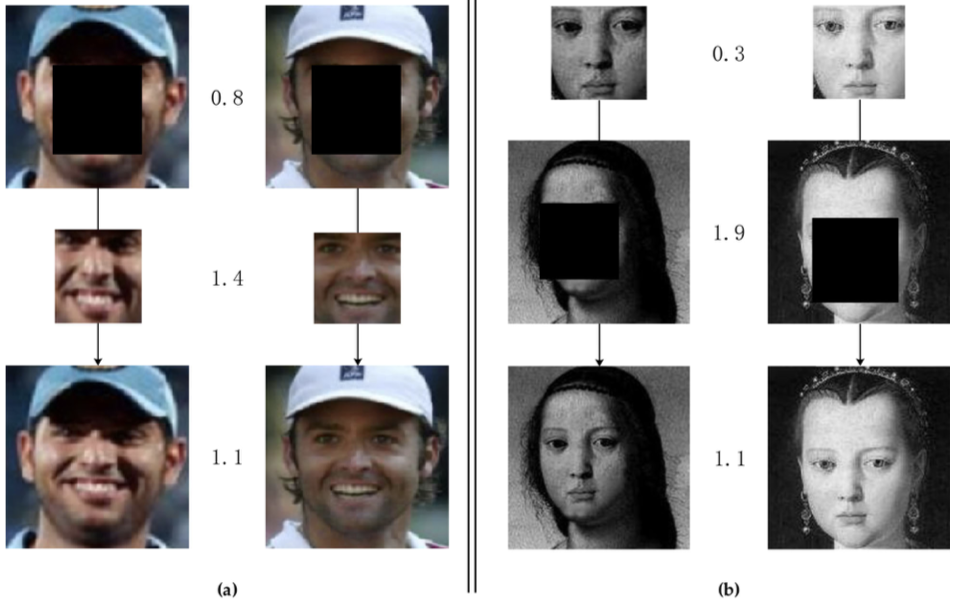
\includegraphics[width = 0.6\linewidth]{images/paper9/importance.png}
        \centering
        \caption{(a) Shows the importance of internal features and (b) shows the importance of external features. The values are the cosine distances.}
        \label{fig:features}
    \end{figure} 
\end{frame}

\begin{frame}{DATASET COLLECTION}
    One of the purposes of this paper is to create a dataset containing similar faces called dataset-similar-face (DSF), in order to test the proposed IE-CNN recognition model with other models. To create the dataset, the following steps were performed:
    \begin{enumerate}
        \item \emph{Collecting The Suitable Data Source}: from LFW and CASIA-WebFace datasets.
        \item \emph{Determining the Similarity Between Two Faces Images}: with distance $L2$ on image vectors.
        \item \emph{Generating the Similar FaceDataset (SFD)}: with images classified in different Grades.
    \end{enumerate}
\end{frame}

\begin{frame}{NETWORK ARCHITECTURE AND TRAINING}
    This paper proposes IE-CNN model which contains two modules to 
    extract internal (local pathway) and external (global pathway) features. 
    The outputs, generated by both pathways, will be merged with a 
    concatenation operation to create a single feature map.
    \begin{figure}[h!]
        \centering
        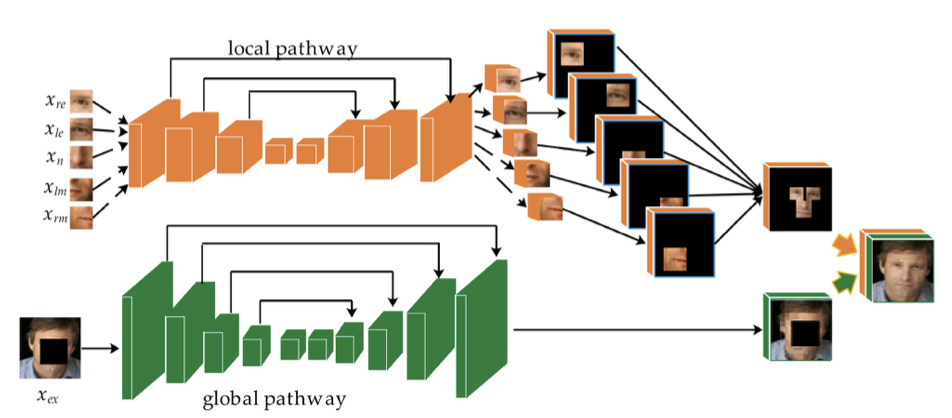
\includegraphics[width = 0.8\linewidth]{images/paper9/IE-CNN.png}
        \centering
        \caption{IE-CNN Architecture.}
        \label{fig:IE-CNN ARCHITECTURE}
    \end{figure}
\end{frame}